\chapter{Background \& Related Work}
\label{chp:background}

In this chapter, the background and related work is discussed. In Section~\ref{sec:background}, fundamental concepts are explained which are used in this thesis. In Section~\ref{sec:related_work} the building blocks are laid out, on which this project has been build.

\section{Background}
\label{sec:background}
% More explanation on the concepts behind the techniques used. Explanation on radar, the chips etc.
% To explain:
% - Heart rate detection methods
% - mmWave technology
% - chirps
% - FFTs
\subsection{Vital sign detection methods}
In this section, a short summary is given about the most common vital signs monitoring systems, and the pro's and cons of each method.

% TODO: add table or image with a summary of all the types mentioned, pro/con

\subsubsection{SpO2 sensors}
The most well known method for measuring heart rate is using a SpO2 sensor. In \cite{sinex1999pulse} the principle of this way of measuring heart rate is explained. This sensor is attached to the finger of a patient. In essence, the sensor consist of two parts: a light emitter and a light detector. The light emitter is located on one side of the finger and emits light, in most cases red LED light and infrared LED light. This light travels through the finger and ends up at the light detector. The light detector measures the light intensity at the detector. A schematic view can be found in Figure~\ref{fig:pulse_oxymeter}. 

This type of sensor works because of a property of hemoglobin. Hemoglobin is located inside of our red blood cells, and stores oxygen to transport it trough the body. A property of hemoglobin is that it absorbs more infrared light if there is a lot of oxygen encapsulated in the hemoglobin. It absorbs more red light if there is a low amount of oxygen encapsulated inside the hemoglobin. This makes it possible to measure the amount of oxygen inside of the body. But, this principle also works in the more general way. Every time the heart beats, blood is pumped in the blood vessels. Because of this pumping behavior, there are constant changes in pressure inside the blood vessels. When fresh blood is pumped inside the blood vessel, there are a lot of red blood cells present and much light, red and infrared, is absorbed. But that blood flows away and there is a period of less blood inside the vessels just before the next heartbeat. At that point in time, there is less light absorbed and more light detected by the detector. Using this principle, the heartrate can be detected.

This method of measuring heartrate of a person is around for more than 40 years, so it is very reliable. The method used is very simple, just a LED and a light detector. This also means that privacy is not a concern, it is only made to detect heartrate and oxygen percentage, but measures nothing else. There are however also some downsides on using an SpO2 sensor. Because it uses a light detector, it could be influenced by the light in the room. Also, this method is less accurate for people with a darker skin color \cite{feiner2007dark}. But the downside which this thesis focuses on is the patient contact. This method only works by having contact with the skin, and having a wire from the sensor on the patient to the device which is processing the data. This could be the cause for discomfort, the patients mobility is decreased because of the wire, and the sensor could fall off. 

% In essence, there are two types of SpO2 sensors, the transmission method and the reflection method. The reflection method is most commonly found on fitness watches and smartwatches. In this setup, the LED and the photo-detector are next to each other. This method makes use of the reflecting properties of the human finger. When the heart beats, more blood is flowing in the finger, and more light is reflected from the LED to the detector. The transmission method is based on the permeable properties of the human finger. The LED is on one side of the finger, the detector is on the other side of the finger. When the heart beats, more blood is present in the finger, and less light is transmitted from the LED through the finger to the detector. Using this principle the heart rate can be measured. This way of measuring is most commonly seen in medical grade equipment.

In more recent research \cite{motin2019selection}, the pulse oximeter sensor can also be used to estimate the breathing rate of a patient. 

\begin{figure}[t]
\centering
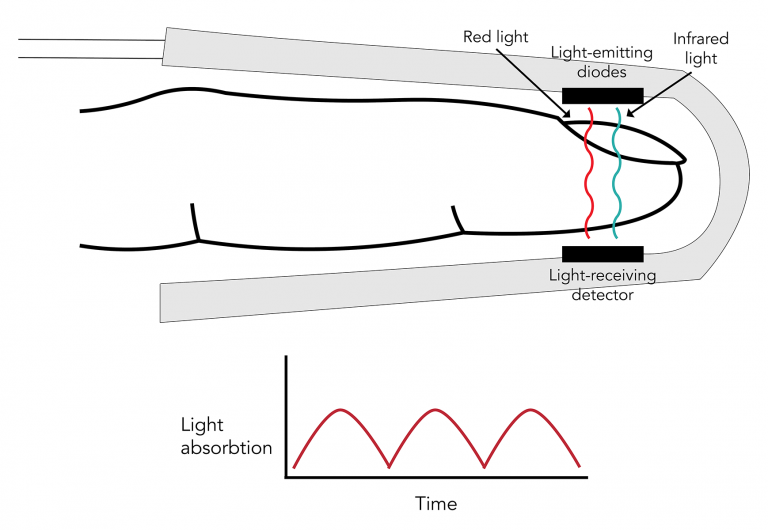
\includegraphics[width=.7\textwidth]{figures/background/pulse_oximeter.png}
\caption{Overview of the parts that make up a SpO2 sensor. The different types of light travel through the finger from the emitter to the detector. From the amount of light arriving at the detector, the graph can be built.}
\label{fig:pulse_oxymeter}
\end{figure}

\subsubsection{ECG monitoring}
Electrocardiogram (ECG) monitoring is a more advanced way of monitoring someones heart rate \cite{berkaya2018survey}. The machine detects and monitors the electrical pulses the heart muscles generate while contracting and relaxing. The detection happens by placing pads on the chest in the heart region, like depicted in Figure~\ref{fig:ecg}. These pads detect the electrical signals generated by the heart muscles. Not only the heart rate can be monitored, but also the order of muscle contraction and the muscle power can be determined, which is beyond the scope of this project. Because the chest also moves using muscles when breathing, the breathing rate can also be determined using some additional processing \cite{charlton2017breathing}.

ECG monitoring is the golden standard in heartrate measurement. This because of the extensive data and information that can be gathered. Doctors heavily rely on ECG's to monitor the heart and diagnose heart problems. There are however some cons that could be considered for this method. ECG's can't be used for very preterm neonates, because they are too small to achieve a reliable reading. ECG's can also not be used for burn victims, because a clean connection to the skin is necessary for the ECG to work. 

\begin{figure}[t]
\centering
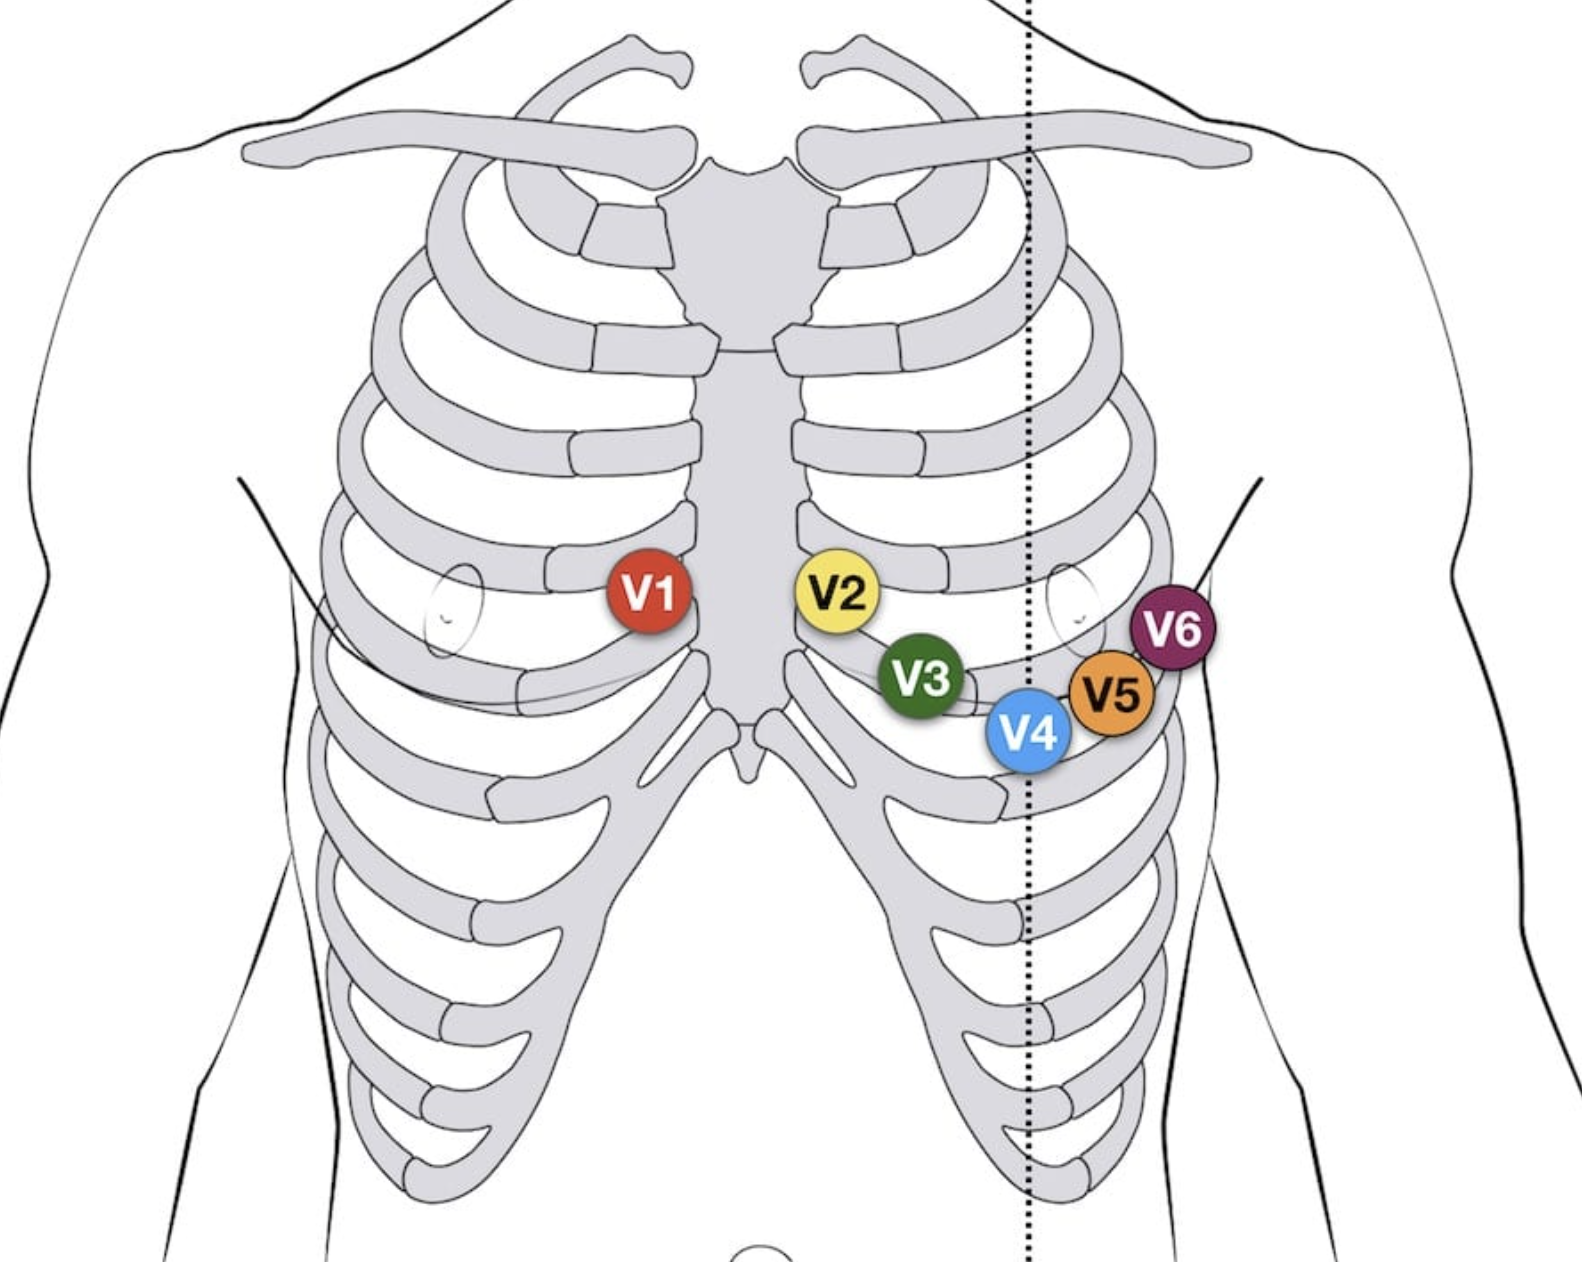
\includegraphics[width=.5\textwidth]{figures/background/ecg.png}
\caption{Placements of the ECG pads on the chest region. These pads can detect the electricity generated by the heart muscles.}
\label{fig:ecg}
\end{figure}

\subsubsection{Vital signs monitoring using radar}
Radar assisted vital signs monitoring is a relatively new research topic. A lot of research is still going on and real world implementations are still very scarce. In Section~\ref{sec:related_work} a overview of the research related to this thesis project is given.  

\subsection{mmWave technology}
\label{sec:mmwave_tech}
The type of radar is a frequency modulated continuous wave (FMCW) radar in the millimeter wave range (30-300GHz), specifically operating in the 60-65 GHz range. The radar module used in this project is the \emph{Texas Instruments IWR6843ISK}, see Figure~\ref{fig:iwr6843isk}. It uses short-wavelength electromagnetic waves with a frequency of typically between 60-81 GHz, which means that it is legal to use in the Netherlands~\cite{freq_plan}. The TI package that is used in this project is an all-in-one solution. It contains the Tx and Rx analog circuitry and antennae, see again Figure~\ref{fig:iwr6843isk}, to generate and capture the RF signals. It also contains analog-to-digital converters (ADCs), microcontrollers (MCUs) and digital signal processors (DSPs) to make signal processing possible all on the chip. It also has some custom hardware accelerators build in to speed up standard radar calculations, such as the generation of fast Fourier transforms (FFTs).

\begin{figure}[t]
\centering
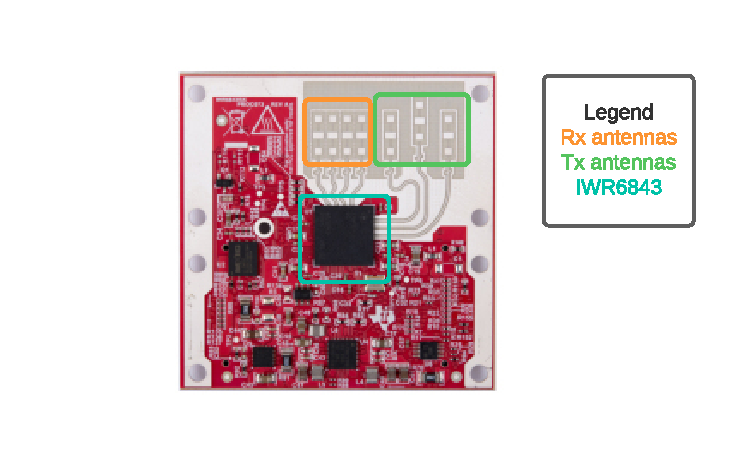
\includegraphics[width=.8\textwidth]{figures/background/IWR6843 legend.pdf}
\caption{The Texas Instruments IWR6843ISK. This module is used throughout the project. See the legend for the most important functional components.}
\label{fig:iwr6843isk}
\end{figure}

A clear difference needs to be made between IWR6843 and IWR6843ISK. The IWR6843 is the chip from TI which is placed on the module, the IWR6843ISK is the module itself, with all of the supporting circuitry and antennae. In Figure~\ref{fig:iwr6843_inner}, the inner components from the IWR6843 can be found. The bottom three antennae are the transmitters. The signal gets generated by the RF front-end and send away by two of the three transmitting antennae. Only the two outermost antennae are used, because the middle antenna is for scanning in one additional dimension. This is why this antenna is slightly elevated, see Figure~\ref{fig:iwr6843isk}. This project only needs 2D radar images, this is why the middle transmitting antenna is not used.

The IWR6843ISK module contains the IWR6843 chip itself, but also the specific antenna configuration, voltage regulators, additional EEPROM chips and temperature sensors, since the chip can get quite hot during operation. See also Figure~\ref{fig:iwr6843_connection} for a functional diagram of the IWR6843ISK module.

\todo{Add a comparision table / why has the IWR6843ISK been chosen as module?}

\begin{figure}[t]
\centering
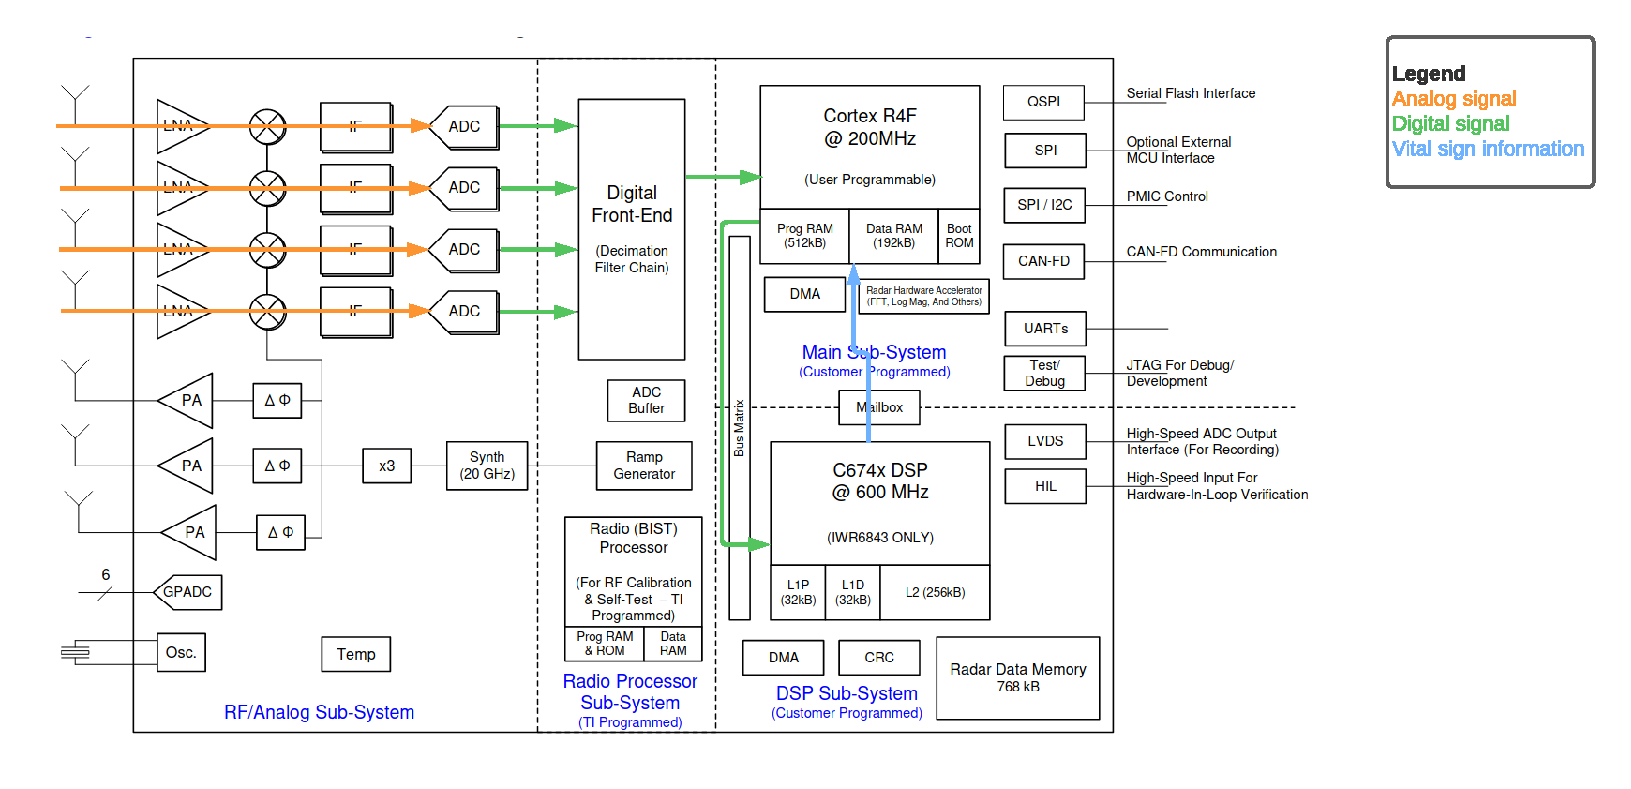
\includegraphics[width=\textwidth]{figures/background/IWR inner.pdf}
\caption{The inner components of the IWR6843. The path the signal takes trough the chip is displayed.}
\label{fig:iwr6843_inner}
\end{figure}

\begin{figure}[t]
\centering
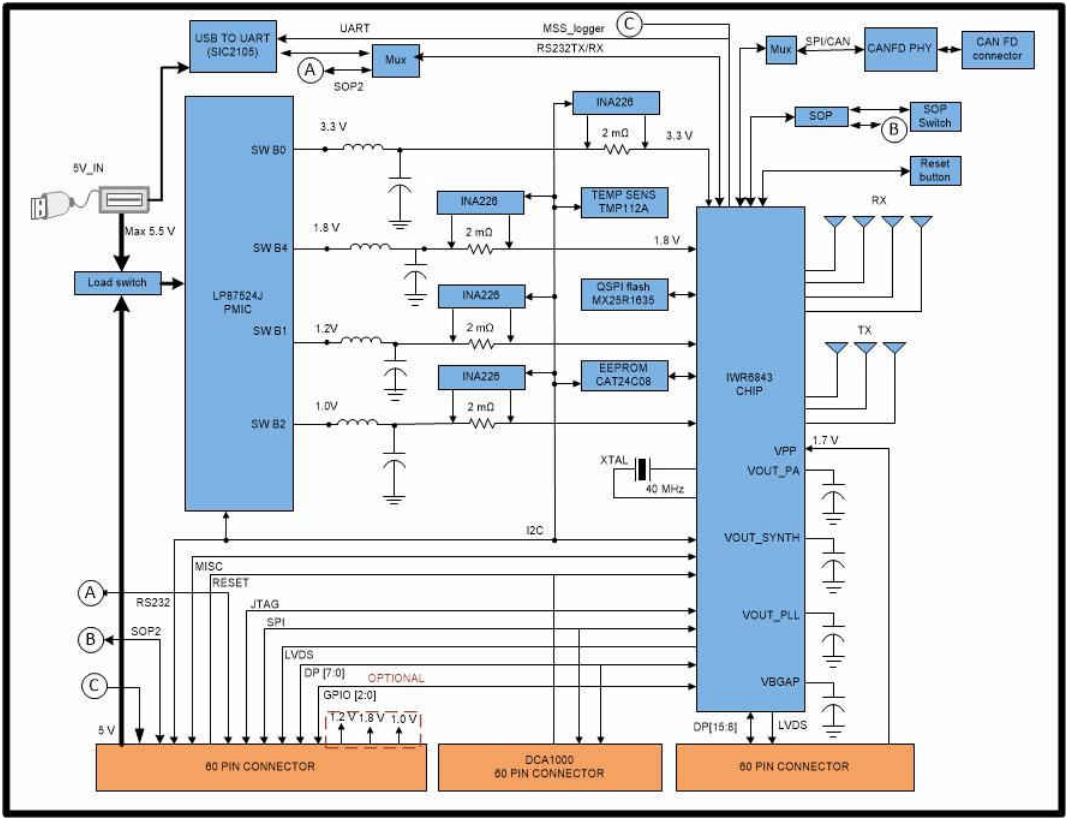
\includegraphics[width=\textwidth]{figures/background/iwr6843isk_connection.png}
\caption{Functional diagram of how the IWR6843 is fitted in the IWR6843ISK module.}
\label{fig:iwr6843_connection}
\end{figure}

\subsubsection{FMCW millimeter wave radar}
Millimeter wave radar is implemented on top of FMCW. Like the name implies, the frequency of these waves is in the range of 30-300 GHz, which means that the wavelength is in millimeters. This property makes these kinds waves a perfect fit for the detection of small objects.
The fundamental concept in radar systems is the transmission of an electromagnetic signal, which is reflected on a target and then received by the radar again. FMCW radars make use of a modulation technique. The frequency of the signal increases linearly over time. One frequency sweep is also called a chirp. 

See Figure~\ref{fig:chirp} for an example chirp waveform, with on the y-axis the magnitude and on the x-axis time. Chirps can be defined by three parameters: frequency ($f_c$), bandwidth ($B$) and duration ($T_c$). A chirp has also a slope ($S$), which captures the rate of change of frequency. These variables can also be found in Figure~\ref{fig:chirpfreqtime}.

\begin{figure}[t]
\centering
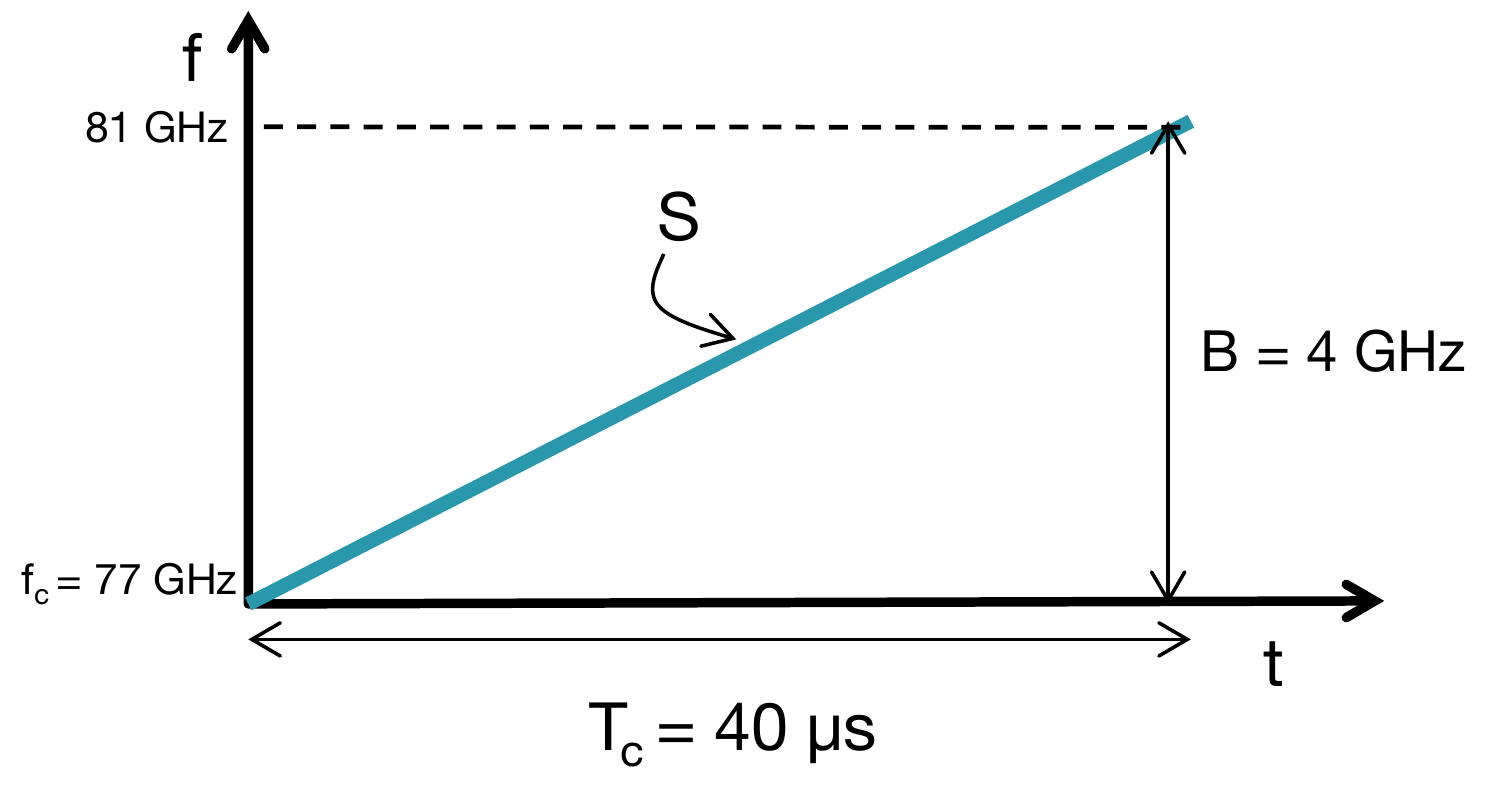
\includegraphics[width=.5\textwidth]{figures/background/chirp_params.png}
\caption{Example frequency/time graph of a chirp. The different variables of the chirp are labeled.}
\label{fig:chirpfreqtime}
\end{figure}

These parameters and more can be programmed in such a way, that the radar waves which are send and received are tuned to the needs of the application. There are three building blocks involved, which can all be defined on their own and connected to each other. See for a visual representation Figure~\ref{fig:chirpframeprofile}.

\begin{itemize}
    \item \textbf{Frame}: the frame is the most high-level building block, and contains one or multiple chirps. The frame also defines how many times chirps need to be looped, how many frames the chip should execute and the frame periodicity.
    \item \textbf{Chirp}: a frame can contain multiple chirps, but a chirp can only contain one profile. A chirp itself only contains a selector for which antennae to use, the rest of the properties of a chirp are defined in a profile. This makes it easier to use the same profile in multiple different chirps.
    \item \textbf{Profile}: the profile contains parameters to define the chirp shape, such as the start frequency of the chirp, the chirp slope but also how many ADC samples needs to be taken during the execution of the chirp.
\end{itemize}

\begin{figure}[t]
\centering
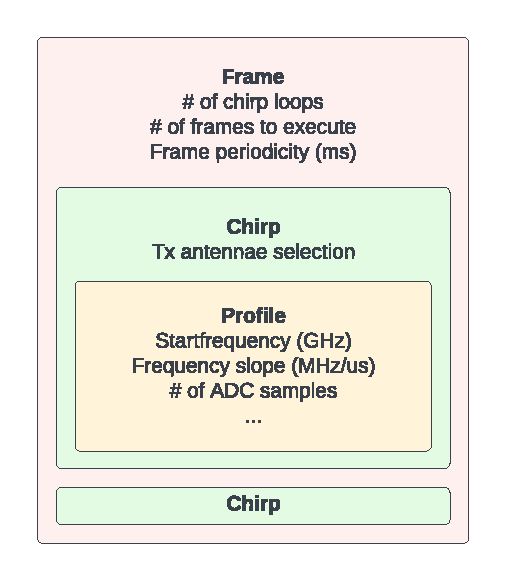
\includegraphics[width=.5\textwidth]{figures/background/chirp frame profile.pdf}
\caption{The relations between a frame, chirp and profile, along with the most important properties of each element. See \cite{mmwavesdk_website} for detailed information.}
\label{fig:chirpframeprofile}
\end{figure}

Many parameters are available to modify the chirp for specific applications, for multiple persons vital signs application, only these variables were the focus: range and resolution. Range is the distance from the radar to the target, measured along the line of sight. For this application both the minimum and the maximum range are important. Resolution is the minimum distance between two targets that permits them to be distinguished by the radar. A balance needs to be found between range and resolution. The signals from the sensor can reach up to 150 meters away, but the resolution will drop to around 4 centimeters. When the sensor is setup to have a range of 2 meters, the resolution can be as low as a couple of millimeters. The balance between maximum range and resolution is important for the multiple people tracking functionality. For the vital signs estimation, the minimum range is important. 

\begin{figure}[t]
\centering
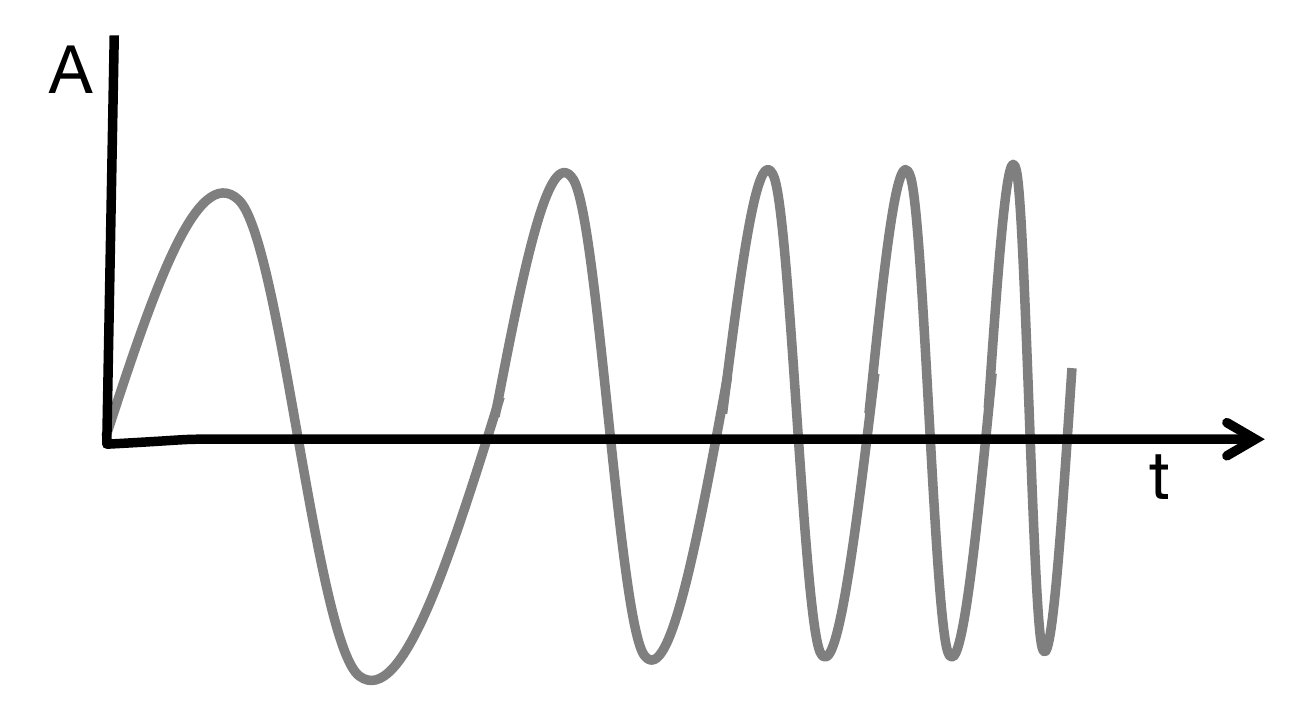
\includegraphics[width=.5\textwidth]{figures/background/chirp.png}
\caption{Chirp signal, with the amplitude as a function over time.}
\label{fig:chirp}
\end{figure}

\subsection{Range estimation}
In Figure~\ref{fig:fmcw_inner}, a scheme of the inner workings of the FMCW chip can be found. First, a chirp is generated using a ramp generator and then mixed with a synthesizer (1) to generate a 20 GHz signal, which is then multiplied to get a 60 GHz signal. This chirp is then transmitted over one or multiple Tx antenna (2). When reflected on an object, the signal returns and is captured using the Rx antenna (3). During the travel of the signal, the frequency shifts. The further the object is away from the sensor, the more the frequency is shifting. The signal from the synth and the received signal from the Rx antenna get mixed (4). This mixer has two signals as input, and one signal as an output. The mixer outputs a signal with a frequency which is the difference between the two input frequencies. This output signal is called the intermediate frequency (IF) signal. In Figure~\ref{fig:if_signal} the situation is displayed more visually. Using this information we can use the equation

\begin{equation}
\tau = \frac{2d}{c}
\label{eq:range_equation}
\end{equation}

where $\tau$ is the time delay and $c$ is the speed of light, to compute the distance to the object $d$. 

This is an example where only one object is used. But in the real world, there are almost always more objects to be detected. All of these objects return another reflection, which means that one transmitted signal from the Tx antenna can result in multiple reflections reaching the Rx antenna, as depicted in Figure~\ref{fig:if_multiple}. In this instance, there are multiple IF tones at once, one for each reflected object. To differentiate between those, we make use of a Fourier transform. After processing this Fourier transform, it results in a frequency spectrum in which each peak will point to one separate IF frequency. The IWR6843 has a hardware accelerator to speed up the Fourier transform generation.

% TODO: calculations for distance in meters using FFT?

\begin{figure}[t]
\centering
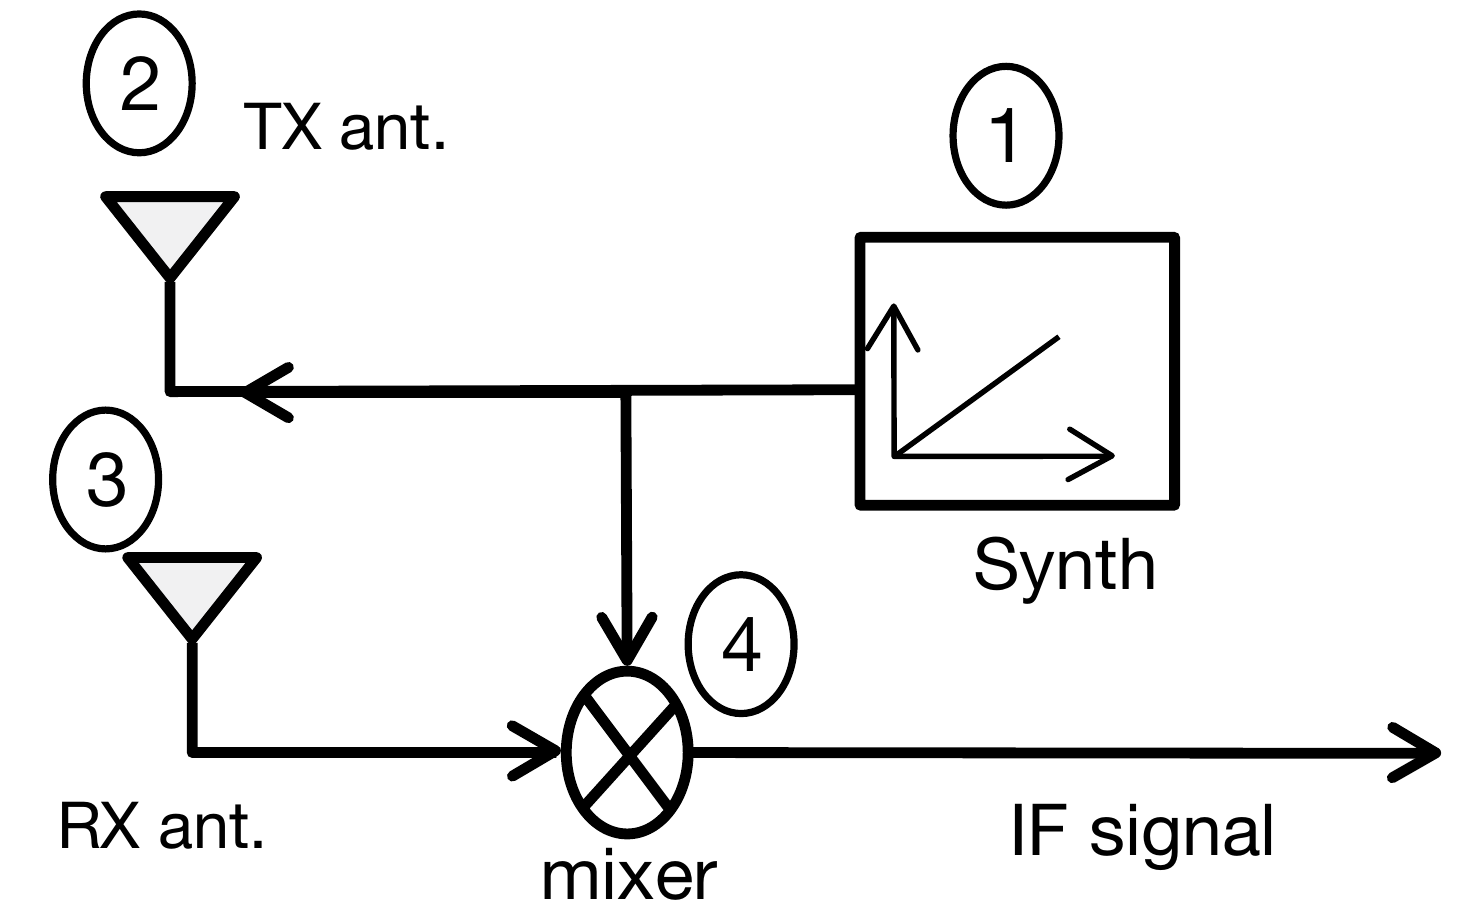
\includegraphics[width=.5\textwidth]{figures/background/fmcw_internals.png}
\caption{Scheme of the inner workings of the FMCW chip.}
\label{fig:fmcw_inner}
\end{figure}

\begin{figure}[t]
\centering
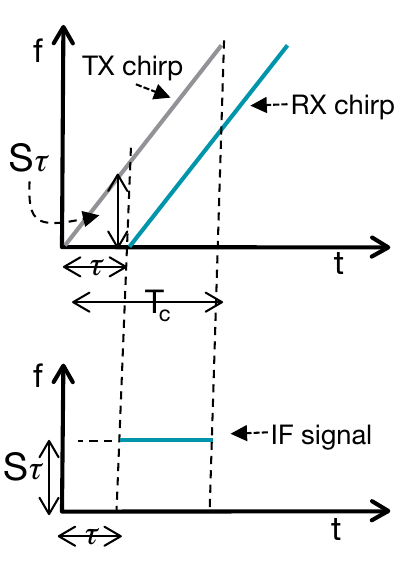
\includegraphics[width=.5\textwidth]{figures/background/if_signal.png}
\caption{The calculation of the IF signal. In the top graph, the Tx and Rx chirp are plotted. In the bottom graph, the IF signal is plotted.}
\label{fig:if_signal}
\end{figure}

\begin{figure}[t]
\centering
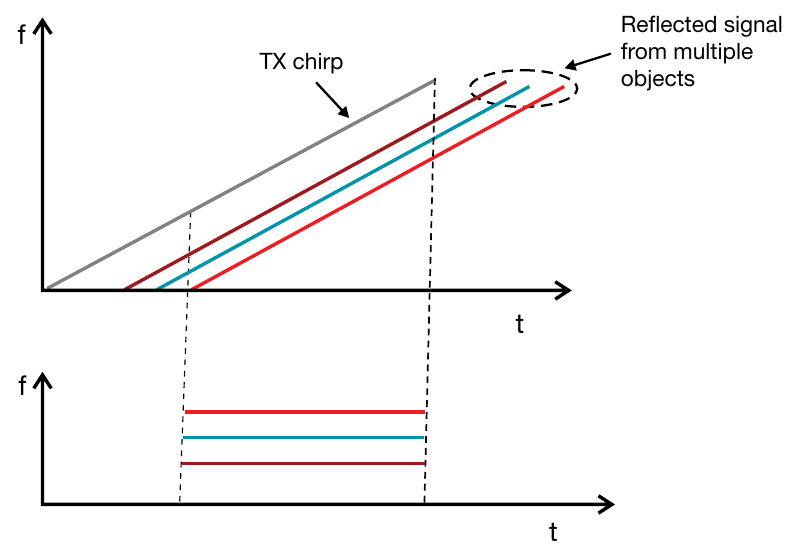
\includegraphics[width=.5\textwidth]{figures/background/reflected_signals.png}
\caption{One Tx signal can result in multiple reflections on the Rx antennas from multiple objects in front of the sensor.}
\label{fig:if_multiple}
\end{figure}

\subsection{Doppler estimation}
The range information, calculated using the range-FFT, is also known as the 1D-FFT. Most of the time, this is the first processing step for radar data. But, there is more information we can extract from the radar data. Sometimes it is useful to know the velocity of objects. This can be done by generating a doppler-FFT. The doppler effect is the change in frequency of a wave in relation to an observer who is moving relative to the wave source.

To calculate the velocity of objects, we need the data from the range-FFT. The radar transmits two chirps, spaced $T_c$ apart from each other. Both of these chirps get reflected on the object and for both of them a range-FFT is calculated. Because the chirps are transmitted almost immediately after each other, the two FFTs have peaks in the exact same location. What matters now is the phase of the peaks. The output of a FFT is an array of complex numbers. The real part says something about the frequency of the signal, the imaginary part says something about the phase of the sinusoidal signal. The phase between the two chirps is changed slightly because even between those two chirps spaced $T_c$ apart, the object moved. The velocity can be derived using this formula:

\begin{equation}
v = \frac{\lambda \Delta \phi}{4 \pi T_c}
\label{eq:doppler_equation}
\end{equation}

Because the velocity is dependent on the phase value, the velocity could wrap around if the object is moving too fast. Therefore, the maximum speed the radar is able to record before the measurements start to be untrustworthy, is:

\begin{equation}
v_{max} = \frac{\lambda}{4 T_c}
\label{eq:doppler_equation_max_speed}
\end{equation}

To determine the velocities of multiple objects, a FFT is used to differentiate between multiple objects. In the example above for only one object, two chirps are needed to calculate the velocity of the object. To distinguish between multiple objects, more chirps are needed. Each chirp is one input data element for the FFT, so the more chirps, the more accurate the result. All of those chirps together forming the data for the range-FFT and the doppler-FFT are called a frame. 

\subsection{Angle estimation}
\label{sec:angle_estimation}
Using the methods above, we can estimate the range and the velocity of multiple objects using range- and doppler-FFTs. But, there is still one more shortcoming of these calculations. They only work for one dimension. This means that if object 1 is 3 meters from the sensor and object 2 is 5 meters from the sensor, everything is fine. But, if two objects are at the same distance to the sensor but with a different angle, these two objects would get merged into one. The solution to this problem is to try and calculate the angle of the object with respect to the sensor, also known as the Angle of Arrival (AoA). This way, the data collection from the sensor can be expanded from one dimension into two dimensions.

To calculate the Angle of Arrival, multiple Rx antennas are needed. In Figure~\ref{fig:angle_estimation} the functional diagram of how angle estimation works is displayed. A chirp is emitted from a Tx antenna. The chirp is reflected on an object and received by the first Rx antenna. The distance between the object and the Rx antenna is $d$. When the signal arrives at the second Rx antenna, it has traveled $d + \Delta d$. Because of this $\Delta d$, the phase on the second Rx antenna is different from the first Rx antenna. A similar formula as the doppler estimation can be formed to tie these concepts together:

\begin{equation}
\Delta \phi = \frac{2 \pi \Delta d}{\lambda}
\label{eq:angle_equation}
\end{equation}

Using some basic geometry, we can deduce the formula for the angle of arrival using Eq. \ref{eq:angle_equation}:

\begin{equation}
\theta = \arcsin{\frac{\lambda \Delta \phi}{2 \pi l}}
\label{eq:angle_equation_2}
\end{equation}

Using multiple Rx antennas, in the case of this project using the IWR6843ISK there are 4 antennas, we can calculate the AoA of different objects using a FFT. At this point, a 2D heatmap can be constructed using the calculations from the different estimations above. This heatmap is the starting point for this project.

\begin{figure}[t]
\centering
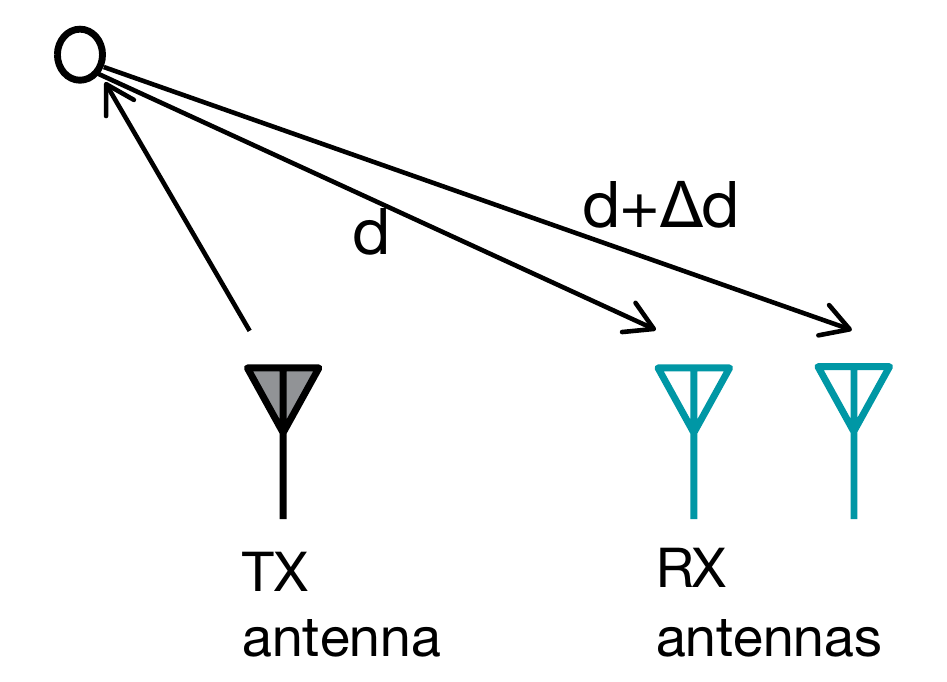
\includegraphics[width=.5\textwidth]{figures/background/angle_estimation.png}
\caption{One Tx signal is received by multiple Rx antennas. Because the signal travels $\Delta d$ longer to one Rx antenna compared to the other, the angle of arrival can be calculated.}
\label{fig:angle_estimation}
\end{figure}

\section{Related Work}
\label{sec:related_work}
% Use building blocks for the related work. What is new? So start with app1, app2 and app3, and based on these you end up with app4. With app4 you define something novel for example. So, describe this path
% Papers to use:
% - Monitoring Vital Signs Using Millimeter Wave \cite{yang2016monitoring}
% - Vital signs monitoring of multiple people using a FMCW millimeter-wave sensor \cite{ahmad2018vital}
% - Radar remote monitoring of vital signs \cite{li2009radar}
Using radar to estimate vital signs has already been researched before. One of the first papers about the subject is \cite{li2009radar}, which uses a transmitter to send a unmodulated signal to a patient and receive the modulated signal back. The signal gets demodulated and the heart rate and breathing rate can be extracted. In this attempt, a lot of analog hardware is used to make the vital signs extraction work. 

A similar attempt has been made by \cite{yang2016monitoring}. The researchers made use of two separate antennas, one for transmitting and one for receiving. The transmitting antenna does a first sweep through the room by physically moving the antenna to detect persons in the room. After that, the transmitter and receiver can zone in on the person and detect the vital signs of that person. The transmitting and receiving is done with large pieces of equipment. 

In \cite{alizadeh2019remote} the step to FMCW radars can be observed. The authors also use a chip from TI, but an earlier model. They make use of a range-FFT to detect a person, and perform vital signs estimation on that person. A disadvantage of this approach is that the solution is only able to estimate the vital signs of one person. Another disadvantage is that the data gathered by the sensor is send to a computer for processing at a later time. This means that the vital signs estimation is not real time. 

The paper which is closest to the research topic of this paper, is \cite{ahmad2018vital}. The authors from this paper all work for TI, and made a proof of concept solution for multiple person vital signs estimation using a TI sensor. The sensor first looks for persons in the 2D space before the sensor. Then, it uses a post-processing beamforming technique to isolate the data for one person at a time to extract the vital signs. It does this for all of the persons within reach of the sensor. Again, there are some disadvantages with this method. Firstly, the beamforming technique they are using to isolate the different persons from each other is not shown in detail. The most important disadvantage is that the calculations are done in Matlab after the data gathering. First, the data is recorded using the DCA1000EVM. Then this data is transferred to a computer and after that the data is processed in post using Matlab. In the medical world, it is important to have information about a patient right away, and not minutes to hours after they have been recorded. \todo{Expand this section}